\documentclass[conference]{IEEEtran}
\IEEEoverridecommandlockouts
\usepackage{cite}
\usepackage{amsmath,amssymb,amsfonts}
\usepackage{graphicx}
\usepackage{textcomp}
\usepackage{xcolor}
\usepackage{booktabs}
\usepackage{multirow}
\usepackage{listings}
\usepackage{float}
\usepackage{tikz}
\usepackage{pgfplots}
\usepackage{acro}
\usepackage[colorinlistoftodos]{todonotes}
\usetikzlibrary{positioning,arrows.meta}
\pgfplotsset{compat=1.17}

\DeclareAcronym{sast}{
  short = SAST,
  long  = static application security testing,
}

\DeclareAcronym{sarif}{
  short = SARIF,
  long  = static analysis results interchange format,
}

\DeclareAcronym{fp}{
  short = FP,
  long  = false positive,
  long-plural-form = false positives,
}

\DeclareAcronym{llm}{
  short = LLM,
  long  = Large Language Model,
  long-plural-form = Large Language Models,
}

\DeclareAcronym{tp}{
  short = TP,
  long  = true positive,
  long-plural-form = true positives,
}

\DeclareAcronym{cwe}{
  short = CWE,
  long  = Common Weakness Enumeration,
}

\DeclareAcronym{mcc}{
  short = MCC,
  long  = Matthews Correlation Coefficient,
}


% Listing float, so that code blocks are numbered as "Listing N".
\newfloat{listing}{tbp}{lol}
\floatname{listing}{Listing}

\lstset{
  basicstyle=\ttfamily\scriptsize\linespread{0.9}\selectfont,
  breaklines=true,
  breakindent=0pt,
  columns=fullflexible,
  keepspaces=true,
  frame=none,
  aboveskip=0pt,
  belowskip=0pt,
  xleftmargin=0pt,
}

% Palette of the metric bars (matches the original figure).
\definecolor{cacc}{HTML}{4C72B0}
\definecolor{cprec}{HTML}{DD8452}
\definecolor{crec}{HTML}{55A868}
\definecolor{cff1}{HTML}{C44E52}

\newcommand{\fk}[1]{\todo[inline, color=green]{\textbf{FK:} #1}}

\begin{document}

\title{Polygraph: Automated False-Positive Classification of SAST Findings}

\author{
\IEEEauthorblockN{Alexander Braml}
\IEEEauthorblockA{\textit{Chair of Computer Engineering} \\
\textit{University of Passau}\\
Passau, Germany \\
alexander.braml@uni-passau.de}
\and
\IEEEauthorblockN{Florian Frank}
\IEEEauthorblockA{\textit{Chair of Computer Engineering} \\
\textit{University of Passau}\\
Passau, Germany \\
florian.frank@uni-passau.de}
\and
\IEEEauthorblockN{Felix Klement}
\IEEEauthorblockA{\textit{Chair of Computer Engineering} \\
\textit{University of Passau}\\
Passau, Germany \\
felix.klement@uni-passau.de}
}

\maketitle

\begin{abstract}
\Ac{sast} tools frequently generate findings
that, upon further investigation, turn out to be \acp{fp} rather than
genuine vulnerabilities. Triaging these \acp{fp} by hand is slow and
draws effort away from the real weaknesses that demand attention. In
this work, we present Polygraph, a tool that classifies each \ac{sast} finding as
a \ac{tp} or an \ac{fp}. It reads and writes reports in standard \ac{sarif}
format and operates between any compliant scanner and viewer. For each finding,
it assembles a compact, finding-specific context from the surrounding code,
together with a data-flow analysis that traces how input reaches the affected
location. It then queries a \ac{llm} for a verdict. When this static
context does not settle a finding, Polygraph escalates it to an autonomous agent
that explores the repository directly. Evaluated with four open-weight \acp{llm}
on the synthetic OWASP Benchmark for Python, Polygraph suppresses 95.8\% of
its \ac{fp} traps at a suppression precision of 0.997 and a
dangerous-suppression rate of 0.4\%, for an F1-score of 0.977 and a balanced
accuracy of 0.973. On RealVuln, a corpus of real-world vulnerable applications
whose findings depend on code spread across a repository rather than a single
file, it reaches a lower F1-score of 0.797 at a balanced accuracy of 0.880,
suppressing 82.5\% of its traps at a dangerous-suppression rate of 5.0\%.
Since these results hold with locally hosted, open-weight models that keep
code from leaving an organization's own infrastructure, Polygraph makes a
reliable source of \ac{sast} triage decisions available even in
security-sensitive settings that cannot rely on third-party inference
providers.
\end{abstract}

\begin{IEEEkeywords}
Static Application Security Testing, SAST, False-Positive Reduction, Software
Security
\end{IEEEkeywords}

\section{Introduction}

With the rise of agentic development workflows, source code is produced at an unprecedented speed, resulting in faster release cycles, while simultaneously increasing the manual code review load.
Code produced by coding agents frequently contains exploitable weaknesses even when functionally correct \cite{vero2025}, and manual security assessment, adding to the burden of functional code review, does not scale with the rate at which such code is produced. \ac{sast} therefore serves as an increasingly important safeguard, inspecting source code without executing it to find potential vulnerabilities before they reach production.

A recurring problem is that a
large share of reported findings does not correspond to a real vulnerability in
its specific context. These \acp{fp} carry a measurable cost. According to a 2025
industry report, 63\% of security teams spend at least four hours per week
triaging \acp{fp} \cite{nash2025falsepositive}. Time spent dismissing
false alerts is time not spent on real vulnerabilities, and a steady stream
of noise erodes developer trust in the tools themselves \cite{johnson2013why}.

Reducing this burden remains difficult by conventional means. Whether a given
finding is an \ac{fp} can rarely be determined from the finding alone. It
also depends on things like how the surrounding code uses the flagged construct or whether
user input can reach it without being sanitized first. A static scanner reports
the finding because it cannot resolve this context on its own, so a
deterministic filter layered on top would have to reconstruct this semantic
understanding the scanner lacks. An \ac{llm} can reason over
this kind of code context, which makes it a suitable basis for this task.

This paper presents Polygraph, a tool that classifies \ac{sast} findings as \acp{tp} or \acp{fp}. This reduces the effort necessary to deal with large volumes of \ac{sast} findings and allows developers to focus on genuine vulnerabilities, directly solving the problems conventional scanners introduce.

Polygraph reads and writes standard \ac{sarif} reports, so it sits between any
compliant scanner and viewer. It parses the heterogeneous set of findings, de-duplicates them based on the type of the finding and location, and categorizes them into \ac{cwe} classes.
Afterwards, it assembles finding-specific contexts that include the surrounding code, documentation and on-demand data-flow analysis, and queries an \ac{llm} for a
verdict. When the static context does not suffice for a decision, the model
declines to classify, and Polygraph escalates the finding to
an autonomous agent that explores the repository directly.

On the OWASP Benchmark for Python \cite{owaspbenchmark}, Polygraph reaches an
F1-score of 0.977 on the \ac{fp} class at a balanced accuracy of
0.973, suppressing 95.8\% of the benchmark's \ac{fp} traps at a
suppression precision of 0.997 and a dangerous-suppression rate of only
0.4\%. RealVuln \cite{realvuln} is a benchmark of intentionally vulnerable
open-source applications whose findings, unlike OWASP's single-file cases,
depend on code distributed across a repository. It is correspondingly
harder: Polygraph reaches a lower F1-score of 0.797 at a balanced accuracy of
0.880. It still suppresses 82.5\% of the benchmark's \ac{fp} traps,
at a dangerous-suppression rate of 5.0\%.

In summary, this paper makes the following contributions:
\begin{itemize}
    \item Polygraph, a \ac{sarif}-native tool that assembles a finding-specific context from surrounding code, documentation, and on-demand data-flow analysis, and queries an \ac{llm} to classify each finding as a \ac{tp} or \ac{fp}, so it drops into any pipeline between an existing scanner and viewer.
    \item A two-stage classification design in which findings the static context cannot settle are escalated to an autonomous agent that explores the repository directly, keeping the common case cheap while still resolving the harder, context-dependent cases.
    \item An evaluation on the OWASP Benchmark for Python and on RealVuln, a repository-scale benchmark of intentionally vulnerable open-source applications, showing that Polygraph suppresses 95.8\% and 82.5\% of each benchmark's \ac{fp} traps, respectively, while keeping the rate of dangerously suppressed \acp{tp} at 0.4\% and 5.0\%.
\end{itemize}

\subsection{Background}

\ac{sast} tools statically analyze a program's source or compiled code and
report code patterns that may indicate a security vulnerability, such as an
injection flaw or unsafe handling of user input \cite{chess2004static}. Each
issue such a tool reports is a finding, annotated with a rule identifier, a
severity, and the code location it concerns. Because these tools only statically
analyze the source code and do not interpret the context around the finding, like sanitization steps or dynamic behavior at runtime, they also report many findings that are not real vulnerabilities in their context.
Some tools also over-approximate and would rather report an \ac{fp} than missing a \ac{tp}, which results in further increases of the overall volume of findings.

Individual \ac{sast} tools historically output their results in incompatible,
proprietary formats, which complicates aggregating and processing findings
across tools. \Ac{sarif} addresses this as an OASIS standard that defines a single
JSON-based format for static-analysis output \cite{sarif2020}. A \ac{sarif} report
records each finding together with its rule, severity, and location, and it
provides standard fields such as \texttt{suppressions} to mark findings that a
viewer should hide. Polygraph reads \ac{sarif} as input and writes \ac{sarif} as output,
which lets it operate between existing scanners and any viewer or dashboard that
supports \ac{sarif}.

Many \ac{sast} findings deal with uncontrolled and unsanitized user input reaching a sensitive sink, such as a database query or system command. For these findings, the way data flows into the vulnerable line is essential
to determine if it is genuine. Data-flow analysis addresses this by statically tracing values from their source, where the data enters the program, to the sink, which in our case is the location reported by the \ac{sast} tool.
A common form is taint analysis, which tracks whether data from an untrusted source, like user input, reaches a
security-sensitive sink, such as a database query, and whether a sanitizer
neutralizes the data along the way \cite{tripp2009taj}.
Polygraph computes this information using \texttt{CodeQL}\cite{codeql}, a well-established framework for semantic code analysis that models a program as a queryable database and includes data-flow and taint-tracking libraries.

\section{Related Work}

ZeroFalse and QASecClaw are the two systems most closely related to Polygraph.
Both combine a \ac{sast} scanner with an \ac{llm} that reviews each finding to
decide whether it is a real vulnerability, the same basis Polygraph builds on,
and both decide it in a single pass. Xiong and Zhang instead evaluate autonomous
agents that investigate every finding on their own, which is the second stage
Polygraph applies selectively when necessary.

ZeroFalse \cite{iranmanesh2025zerofalseimprovingprecisionstatic} operates only
on findings from CodeQL. It treats such alerts as structured contracts and
enriches them with the scanner's own data-flow trace, the surrounding code, and
information specific to each \ac{cwe} class before a
single \ac{llm} pass returns a verdict. Across the OWASP Java Benchmark and a curated
real-world dataset it reaches F1-scores of 0.912 and 0.955, below Polygraph's
0.977 on the Python variant of the OWASP Benchmark. Its design is based
on \ac{cwe}-specific tailoring, and the authors name contextual blindness, the
difficulty of supplying sufficient context for a multi-file finding, as an open
problem. Polygraph addresses this problem with the autonomous escalation agent that gathers evidence on-demand.
It also maintains no prompt per weakness class, but uses a generic
prompt template for all findings that includes a description of the concrete
finding. Furthermore, rather than reuse the data-flow traces the scanner potentially
emitted, Polygraph computes its own taint analysis on-demand,
which removes the dependence on a scanner that populates \ac{sarif} flow traces
comprehensively. ZeroFalse depends on CodeQL for exactly this reason. As a
result, it cannot triage findings of arbitrary scanners, while Polygraph sits
between any \ac{sarif}-compatible scanner and viewer.

QASecClaw \cite{ameen2026qasecclawmultiagentllmapproach} orchestrates several
role-specific agents that cover scan planning, Semgrep-based scanning, evidence
correlation, and an \ac{llm} \ac{sast} Filter Agent. It classifies each finding from its
enclosing source file and \ac{cwe} label, with a fail-open policy that retains a
finding whenever the model fails. On OWASP Benchmark v1.2 it achieves an F1-score
of 0.909 and removes 88.6\% of \acp{fp}. Its filter, however,
performs no data-flow analysis and reasons only over the enclosing file. Its
agents also form a fixed pipeline rather than an investigator that gathers
missing evidence when needed. In contrast, on the Python variant of the OWASP Benchmark,
Polygraph reaches an F1-score of 0.977 while suppressing 95.8\% of the \ac{fp} traps.

Xiong and Zhang \cite{xiong2026} evaluate three general-purpose coding agents,
Aider, OpenHands, and SWE-agent, as \ac{fp} filters under three different
models, rather than proposing a system of their own. Each agent receives the
alert and the source code and settles the finding on its own. On OWASP Benchmark
v1.2 for Java they reduce an initial \ac{fp} rate of 98.3\% to 6.3\%, and the
result carries over to C/C++ findings.

ZeroFalse and QASecClaw judge every finding in a single, fixed-context pass, and
neither recovers when the evidence a verdict needs is missing from that context.
Xiong and Zhang measure what this costs. A baseline that receives exactly the
files their agent had read, but answers in one pass, reaches an F1-score of
0.516 against the agent's 0.955, so the deciding factor is the iterative
gathering of evidence rather than a larger context. Polygraph therefore treats
uncertain as a first-class verdict. The cheap first stage answers the findings
it can, and only those it cannot resolve escalate to an autonomous agent that
explores the source code. This confines expensive exploration to the
hard-to-decide cases that the two prior systems leave unresolved, directly
attacks the contextual-blindness limitation that ZeroFalse names, and costs far
less than running an agent on every finding, at 8,196 tokens per OWASP finding on average
against the 130,846 tokens per alert their best configuration needs.

The same design also decides how many real vulnerabilities survive. Their best
configuration classifies 22.25\% of the benchmark's real vulnerabilities as
\acp{fp}, which leads the authors to reject such agents for automatic suppression. Polygraph reaches a
dangerous-suppression rate of 0.4\% on the Python variant of the OWASP benchmark, a different corpus
but the same weakness families, because its escalation trigger is asymmetric. It
fires on every uncertain verdict and every \ac{fp} below high certainty, but
never on a \ac{tp}, so suppression is the only verdict that has to survive a
second pass.

Two further differences widen Polygraph's applicability. All three evaluations
cover Java, ZeroFalse through CodeQL, QASecClaw through Semgrep, and Xiong and
Zhang through four scanners at once and a small C/C++ sample. In contrast,
Polygraph supports Python, C, C++, JavaScript, and TypeScript first-class, but can
also handle findings in other languages. Where ZeroFalse consumes
\ac{sarif} only from CodeQL and QASecClaw consumes Semgrep JSON, Polygraph both reads and
writes regular \ac{sarif}, marking \acp{fp} through the standard
\texttt{suppressions} field. This way, it slots between any compliant scanner
and viewer. A prompt- and tool-hashing cache further makes repeated scans of an
unchanged codebase effectively free, a concern that none of the three addresses.

On their respective OWASP evaluations, ZeroFalse and QASecClaw report F1-scores
of 0.912 and 0.909, while Polygraph reaches 0.977. This gap has two causes.
Polygraph suppresses more \acp{fp} and, at the same time, misclassifies fewer
real vulnerabilities as \acp{fp}, so less noise reaches the reviewer without
more real vulnerabilities being hidden. The agents of Xiong and Zhang achieve
only the first, as they remove a comparable share of the noise but hide far more
real vulnerabilities. Only suppression that is safe in both directions can be
trusted, and that is what lets a team act on Polygraph's verdicts and re-examine
the escalated cases instead of double-checking the whole report.

\section{Approach}

Polygraph takes two inputs: a \ac{sarif} report that lists all findings and the root directory of the analyzed source code. From these, it classifies every finding as a \ac{tp} or an \ac{fp} in a two-stage process and writes the verdicts back into an annotated copy of the report.

\subsection{Architectural Overview}

\begin{figure}[t]
\centering
\begin{tikzpicture}[
  box/.style={draw, rounded corners=2pt, inner sep=4pt, align=center,
              font=\footnotesize, minimum height=6mm},
  arr/.style={-{Stealth[length=4pt]}, semithick},
  lbl/.style={font=\scriptsize, fill=white, inner sep=1.5pt, align=center},
  node distance=6mm,
]
  % --- inputs ---
  \node[box] (sarif) {SARIF report};
  \node[box, right=8mm of sarif] (src) {Source code};
  \path (sarif) -- (src) coordinate[midway] (in);

  % --- pipeline ---
  \node[box, below=8mm of in] (parse) {Parse findings};
  \node[box, below=of parse] (enrich) {Enrich context};
  \node[box, below=of enrich] (class) {Static context\\classification};
  \node[box, below=20mm of class] (out) {Annotated SARIF};
  \node[box, right=26mm of class] (agent) {Escalation\\agent};

  % --- edges ---
  \draw[arr] (sarif) -- (parse);
  \draw[arr] (src)   -- (parse);
  \draw[arr] (parse) -- (enrich);
  \draw[arr] (enrich) -- (class);
  \draw[arr] (class) -- node[lbl, left] {TP / FP} (out);

  \draw[arr] (class.east) to[bend left=12]
        node[lbl, above=1mm, pos=0.5, yshift=0.5mm] {uncertain} (agent.north west);
  \draw[arr] (class.east) to[bend right=12]
        node[lbl, below=1mm, pos=0.5, yshift=-0.5mm]
        {\ac{fp},\\medium / low confidence} (agent.south west);

  \draw[arr] (agent.south) |- node[lbl, above, pos=0.72]
        {TP / FP /\\UNCERTAIN} (out.east);
\end{tikzpicture}
\caption{Overview of the Polygraph pipeline. Findings parsed from the \ac{sarif}
report are enriched with context from the source tree and classified by the
first-stage \ac{llm}. Only findings it marks uncertain or
\ac{fp} with medium or low confidence escalate to the autonomous
agent before Polygraph writes the annotated \ac{sarif} report.}
\label{fig:pipeline}
\end{figure}

The pipeline, shown in Fig.~\ref{fig:pipeline}, first reads and parses the \ac{sarif}
report and then iterates over all findings. For each finding, Polygraph
assembles the required context, renders it into a prompt, and sends the prompt
to the model for classification. Context generation is modular. A new enricher
can extend the context without any change to the surrounding pipeline. Prompt
templates are version-controlled and adjustable, as Polygraph inserts the
context into templates rather than constructing them in code. Model
endpoints are interchangeable as well, and any OpenAI-compatible endpoint is
supported. When the model returns uncertain or \ac{fp}
with medium or low certainty for a finding, Polygraph passes that finding to the
second stage using an autonomous agent.

To keep re-runs cheap and reproducible, Polygraph hashes every rendered prompt
and, with an optional SQLite cache keyed by that hash and model name, skips the
model call for identical prompts. For escalated findings, it hashes the initial
prompt as well as the tool calls and their results, so even the results of these
findings can be efficiently cached. Because context assembly and tool calling are deterministic,
re-scanning an unchanged codebase is effectively free, and across successive
scans only the few newly surfaced findings require classification, while
unchanged findings reuse their earlier verdicts.

Polygraph finally writes a copy of the original \ac{sarif} report, enriched with
additional attributes. For an \ac{fp} it adds the standard \ac{sarif}
\texttt{suppressions} field and records the reasoning behind the decision. For
every finding it additionally adds a custom property that
holds the verdict and the reasoning. A dashboard or \ac{sarif} viewer can read these
attributes to display the verdicts, which lets developers concentrate on the
\acp{tp}.

A central design goal was to keep Polygraph extensible to new languages. Because the
pipeline is language-agnostic, Polygraph works with any language or
technology out of the box, though at a basic level of support. In this default mode,
the \texttt{SnippetEnricher} falls back to extracting a configurable number of lines
above and below the affected line rather than the enclosing method, class, or file, and
the \texttt{DataflowEnricher} is unavailable, so no data-flow analysis is performed.

Raising a language to full support requires two additions. Richer snippet extraction
requires extending the tree-sitter integration to install and import the language's
grammar. Data-flow analysis requires a new custom query. \texttt{CodeQL}, the framework
we use for this purpose, is language-agnostic in principle but still relies on
language-specific queries. Polygraph currently provides full support for Python, C,
C\texttt{++}, JavaScript, and TypeScript, which already covers many of the most
popular languages in use today.

Every stage of the pipeline fails safely. If a finding cannot be classified, because context assembly fails or because the model request errors out, Polygraph keeps it in the resulting report without annotation. A failure therefore never suppresses a finding, so the report remains trustworthy even when parts of the pipeline do not succeed.

\subsection{Stage 1: Static Classification}

The first step in classifying a finding is to assemble the context for the \ac{llm} to use to output a verdict.
This context should be enough to settle a verdict, but, to not confuse the model with too much context, it should be compact. To dynamically generate this context and test different configurations, Polygraph relies on Enrichers, which form the foundation of context generation, and it currently implements three of them. The \texttt{HeaderEnricher} extracts the header comment from the first lines of a file, following the comment syntax of the file's language. The file header often states what the file does, who wrote it and why, which can help the model judge a finding in that file. The \texttt{SnippetEnricher} extracts the code that surrounds the finding. It parses the file with tree-sitter and offers several strategies to extract code context. One can include the enclosing method, class or file or a configurable number of lines above and below the affected line.
The immediately surrounding code is essential for the model to understand what the code does and does not do. A possible SQL injection for example needs to know whether sanitization occurs before user-input reaches a query, which can be checked using the code surrounding the finding.

The \texttt{DataflowEnricher} performs data-flow analysis on all variables on the affected line and shows how data reaches those variables.

Because some tools also scan the git history, all enrichers read the affected file at the exact commit of the finding to get the correct file content. Each enricher also carries a numeric priority, so that a configurable token limit drops low-priority context first. The output of the enrichers is then assembled into a user prompt describing the concrete finding that is to be classified.
The system prompt is static and does not change between findings. It gives instructions on how to classify findings and frames the classification as one question: does the finding's described weakness hold in the shown code? It also provides detailed criteria for tracing sources to sinks and confirming mitigation. The prompt also explicitly steers the model towards uncertain whenever the context is not enough to settle a finding.
This system prompt together with the customized user prompt is then sent to the \ac{llm} for classification. The model then returns structured output containing a verdict, reasoning and a certainty indicating how confident the \ac{llm} is in its answer.

If the model is sure this is an \ac{fp} or \ac{tp}, this verdict is annotated in the resulting \ac{sarif}-report. If the model returns uncertain or \ac{fp} with only a medium or lower certainty, the second stage using the autonomous escalation agent is activated. Activating it also for low- and medium-confidence \acp{fp} as well ensures the model checks this verdict once more with a more-capable model, as suppressing real \acp{tp} is a costly mistake.

\subsection{Stage 2: Autonomous Classification Agent}

Findings that the first stage does not settle are handed to an autonomous
escalation agent that has access to various read-only tools to interact with the source code.
The agent investigates the finding on its own and must commit to the same
structured verdict the first stage returns.

It has access to three read-only tools. \texttt{read\_file} returns a source file with
line numbers, either a requested range or a truncated version of the file
together with information about its size. \texttt{list\_directory} lists the
entries of a directory, and \texttt{search\_files} searches the repository for a
regular expression and returns the matching lines with their locations. Every path
a tool receives is resolved against the repository root and rejected if it escapes it, and each
tool truncates its output so that a single call cannot flood the context
window. A configurable budget of model requests bounds the investigation. If the agent exhausts it, Polygraph reports uncertain, leaving the annotated finding in the report for manual review.

The agent deliberately does not receive the static context of the first stage.
Its user prompt includes only data about the finding as well as the first-stage reasoning, which
names the missing evidence. It also prescribes an "investigate then commit" pattern, where the agent should first gather comprehensive evidence before committing to a verdict.
The system prompt on the other hand includes the agent's role, the available tools and instructions on how to classify findings as well as a set of rules preventing shortcuts. These rules define things like guards only counting as genuine mitigation if their actual implementation was read or secrets that only count as real ones if they are consumed by security-sensitive code.

Caching this stage requires more effort than caching the first, because the
verdict depends on files the prompt does not contain. Polygraph records every
tool call of a run together with a hash of its result. On a later run it replays
the recorded calls against the current source tree and reuses the cached verdict
only if every result reproduces exactly and any deviation triggers a fresh
investigation. These records double as an audit transcript of what the agent
read. The agent's model is configured independently of the first-stage model, so
that the minority of findings reaching this stage can be resolved by a stronger
model and the extra cost arises only where it pays off.

\section{Evaluation}

This evaluation measures how accurately Polygraph classifies \ac{sast} findings as real or \acp{fp}, and how this accuracy varies across different \acp{llm}. At its best, Polygraph reaches an F1-score of 0.977 and a suppression precision of 0.997. The evaluation rests on two open-source benchmarks. The OWASP Benchmark for Python
\cite{owaspbenchmark} contains 1230 test cases, each labeled as real or not.
RealVuln \cite{realvuln} is a collection of intentionally
vulnerable open-source applications. We use its human-authored ground-truth, which comprises 748
findings over 236 files and 73 \acp{cwe}, 622 real vulnerabilities and
126 hand-authored traps that look vulnerable but are not. The distribution of findings in
OWASP is skewed the other way: 452 real vulnerabilities against 778 traps.
Both benchmarks grade detection rather than \ac{fp} classification, so we synthesize one \ac{sarif}-report with one finding for each ground-truth entry. The details of these findings include a basic description, the \ac{cwe} assigned as well as the location of the finding. The assembled report is then passed to Polygraph together with the source code. The source code is cleaned of any ground-truth data, documentation or comments that may hint towards the verdict of a finding. Otherwise the \ac{llm} may base its verdict on the ground-truth data, which would invalidate the evaluation results.

An \ac{fp} verdict is the positive class for precision, recall,
and the F1-score throughout, since detecting \acp{fp} is the goal. Plain
accuracy says little, as the benchmarks are unbalanced in opposite directions.
We therefore report the balanced accuracy and the \ac{mcc}
together with the dangerous-suppression rate
\[
  \frac{\text{real vulnerabilities classified as \acp{fp}}}{\text{real vulnerabilities}},
\]
which indicates how many real vulnerabilities were wrongly suppressed.

Every run uses method-level snippet extraction, the file header enricher, and
no data-flow analysis, and the cache is disabled, so every finding is freshly
classified and timing stays consistent across runs. Both stages use the same model, and escalation follows the
default policy. The rendered prompts are identical across all runs.

Data-flow analysis is the slowest step in practice, taking several minutes even for simple projects,
longer than the model call that follows it. Since its result is needed for
every context and prompt assembly, enabling it renders the cache ineffective.

Four open-weight models classified both benchmarks under an identical prompt and
context configuration, each serving both stages: Qwen 3.8 27B, Gemma 4 31B,
Qwen 3.6 35B, and Qwen3-Next-80B. We chose these four as well-known, readily available models that span a wide range of parameter counts and two model families.
These models can all be hosted locally, which was a deliberate choice. Security-sensitive findings may contain identifying information or sensitive source code, which is better confined to a trusted environment than sent to third-party inference providers. This also reflects deployment reality, as many organizations will not permit code or vulnerability data to leave their infrastructure \cite{khojah2025}, so a pipeline that depends on external APIs would be unusable in these settings.
We served all models locally with vLLM on a machine with two AMD EPYC 7542 CPUs (32 cores each, 64 cores total), 97\,GB of RAM, and 8$\times$NVIDIA RTX A4500 GPUs with 20\,GB of VRAM each.

\subsection{Classification Quality}

Table~\ref{tab:confusion} shows a run over both benchmarks with Qwen 3.8 27B, the best-performing model in our tests. On the OWASP Benchmark, Polygraph suppresses 745 of 778 traps at a suppression
precision of 0.997, for an F1-score of 0.977 at a balanced accuracy of 0.973
and an \ac{mcc} of 0.950. Two of 452 real vulnerabilities were suppressed and 98.9\%
retained.

For RealVuln, suppression recall stays comparable at 0.825, but precision
drops to 0.770, for an F1-score of 0.797 at a balanced accuracy of 0.880 and an
\ac{mcc} of 0.762. Here 31 out of 622 real vulnerabilities were hidden, a dangerous-suppression
rate of 5.0\%.

Performance differs between the two settings. On synthetic single-file cases the pipeline errs rarely, while on real applications, where a verdict depends on code distributed across a repository, roughly one suppression in four is incorrect. Section \ref{sec:model-comparison} analyzes the cases where the classification was wrong and examines the common sources of error.

\begin{table}[t]
\caption{Verdicts of the Qwen 3.8 27B run over both corpora. Rows give the
benchmark label, columns the verdict Polygraph assigned. \texttt{UNCERTAIN}
verdicts (2 on OWASP, 6 on RealVuln) and findings that errored (7 and 6) are
counted in the class sizes but omitted from the columns.}
\label{tab:confusion}
\centering
\footnotesize
\begin{tabular}{lrrrr}
\toprule
& \multicolumn{2}{c}{OWASP} & \multicolumn{2}{c}{RealVuln} \\
\cmidrule(lr){2-3}\cmidrule(lr){4-5}
Oracle & Verdict FP & Verdict TP & Verdict FP & Verdict TP \\
\midrule
Real vulnerability & 2   & 447 & 31 & 581 \\
Trap               & 745 & 27  & 104 & 20  \\
\midrule
Class size & \multicolumn{2}{c}{452 / 778} & \multicolumn{2}{c}{622 / 126} \\
\bottomrule
\end{tabular}
\end{table}

The escalation agent fired on 44 OWASP findings (3.6\%) and 194 RealVuln
findings (26.1\%). Since it triggers only on uncertain verdicts or on
\ac{fp} below high certainty, every escalated finding ending
as \ac{tp} is one the agent overturned. On OWASP it overturned
19, all real vulnerabilities, and correctly confirmed 23 suppressions. On
RealVuln it overturned 152, of which 145 are real vulnerabilities and 7 traps.

\subsection{Model Comparison}
\label{sec:model-comparison}

Fig.~\ref{fig:quality} compares all four models on both benchmarks.
The ranking by F1 is identical in each case, led
by Qwen 3.8 27B, with the three leading models spanning 0.09 F1 on OWASP and
0.11 on RealVuln. Parameter count does not predict quality, as
the 80B model ranks last and the 27B model leads. What separates them is
suppression recall, which spans 0.329 to 0.958 on OWASP while precision there
varies by less than 0.01. Suppression correctness is effectively constant across models, while they vary in how many \acp{fp} they suppress.

\begin{figure}[t]
\centering
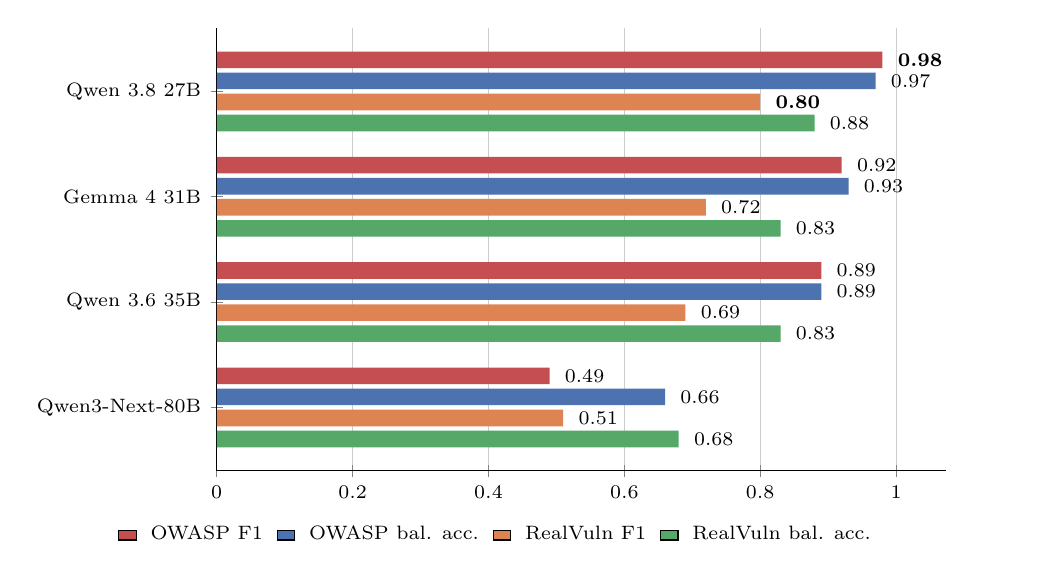
\begin{tikzpicture}
\begin{axis}[
  xbar, bar shift=0pt,
  width=0.97\columnwidth, height=7.2cm,
  enlarge x limits=false,
  xmin=0, xmax=1.18,
  xtick={0,0.2,0.4,0.6,0.8,1.0},
  bar width=6pt,
  % model i sits at y=i (1 = worst, 4 = best), the four bars of a model at
  % y=i+0.30, i+0.10, i-0.10, i-0.30, so OWASP F1 is on top of each group
  ymin=0.4, ymax=4.6,
  ytick={1,2,3,4},
  yticklabels={Qwen3-Next-80B, Qwen 3.6 35B, Gemma 4 31B, Qwen 3.8 27B},
  yticklabel style={font=\scriptsize},
  xticklabel style={font=\scriptsize},
  xmajorgrids, grid style={black!20, very thin},
  axis lines=left,
  axis line style={-},
  x axis line style={shorten >=26pt},
  point meta=explicit symbolic,
  nodes near coords={\pgfplotspointmeta},
  every node near coord/.append style={anchor=west, font=\scriptsize, xshift=2pt},
  legend style={at={(0.35,-0.10)}, anchor=north, legend columns=4,
                font=\scriptsize, draw=none, column sep=3pt,
                /tikz/every even column/.append style={column sep=3pt}},
  legend image code/.code={\draw[#1] (0cm,-0.06cm) rectangle (0.22cm,0.06cm);},
]
\addplot[fill=cff1, draw=none] coordinates {
  (0.98,4.30) [\textbf{0.98}]  (0.92,3.30) [0.92]
  (0.89,2.30) [0.89]           (0.49,1.30) [0.49]
};
\addplot[fill=cacc, draw=none] coordinates {
  (0.97,4.10) [0.97]  (0.93,3.10) [0.93]
  (0.89,2.10) [0.89]  (0.66,1.10) [0.66]
};
\addplot[fill=cprec, draw=none] coordinates {
  (0.80,3.90) [\textbf{0.80}]  (0.72,2.90) [0.72]
  (0.69,1.90) [0.69]           (0.51,0.90) [0.51]
};
\addplot[fill=crec, draw=none] coordinates {
  (0.88,3.70) [0.88]  (0.83,2.70) [0.83]
  (0.83,1.70) [0.83]  (0.68,0.70) [0.68]
};
\legend{OWASP F1, OWASP bal. acc., RealVuln F1, RealVuln bal. acc.}
\end{axis}
\end{tikzpicture}
\caption{F1-score and balanced accuracy of four models on both benchmarks, sorted
by OWASP F1 with the best model on top. F1 refers to the \ac{fp} class.
The best F1-score per benchmark is highlighted.}
\label{fig:quality}
\end{figure}


The models differ in how aggressively they suppress, and this cost of aggressiveness differs between the two benchmarks. On OWASP recall is nearly free: Qwen 3.8 27B catches 95.8\% of traps while hiding 2 of 452 real vulnerabilities. On RealVuln it is not, as recalls of 0.413 to 0.825 come with dangerous-suppression rates of 4.3\% to 8.8\%. The two do not move together strictly, however, since Qwen 3.8 27B reaches the highest recall at 5.0\% while Qwen 3.6 35B hides 8.8\% of the real vulnerabilities for a lower one. Qwen3-Next-80B marks the degenerate end, answering \ac{tp} to almost everything. It therefore has the lowest dangerous-suppression rate on RealVuln, but leaves 522 of 778 OWASP traps in the report.

Cost varies more than quality does (see Table~\ref{tab:cost}), and escalation
frequency drives it, since identical prompts give every model a similar input
volume per call. Gemma 4 31B hands 38.1\% of the RealVuln findings to the agent and
needs 44\% more tokens per finding than the leading model at a lower
F1, whereas Qwen3-Next-80B never escalates on OWASP and is an order of
magnitude faster at the worst F1. Token volume per finding otherwise tracks
escalation rate rather than model size: Qwen3-Next-80B, which escalates
least, is also cheapest in tokens on both benchmarks, while Gemma 4 31B and
Qwen 3.6 35B, which escalate 4 to 9 times as often on RealVuln as on OWASP,
need 2.3 to 3.2 times as many tokens per finding there. Classification is sequential, so per-finding
latency is also throughput: the Qwen 3.8 27B run took 17.5 hours on OWASP and
19.5 on RealVuln.

\begin{table}[t]
\caption{Escalation rate, mean per-finding latency in seconds, and mean
per-finding token volume of the first-stage and escalation calls combined,
measured over all classified findings of each run.}
\label{tab:cost}
\centering
\footnotesize
\begin{tabular}{lrrrrrr}
\toprule
& \multicolumn{3}{c}{OWASP} & \multicolumn{3}{c}{RealVuln} \\
\cmidrule(lr){2-4}\cmidrule(lr){5-7}
Model & Esc. & s & Tokens & Esc. & s & Tokens \\
\midrule
Qwen 3.8 27B    & 3.6\% & 51.4 & 8,196  & 26.1\% & 94.8 & 21,669 \\
Gemma 4 31B     & 4.1\% & 21.2 & 9,857  & 38.1\% & 37.0 & 31,114 \\
Qwen 3.6 35B    & 4.4\% & 26.5 & 10,018 & 19.5\% & 33.0 & 22,719 \\
Qwen3-Next-80B  & 0.0\% &  2.5 & 7,700  &  2.9\% &  4.9 &  9,182 \\
\bottomrule
\end{tabular}
\end{table}

\subsection{What the Models Get Wrong}
\label{sec:error-analysis}

Of the 27 OWASP traps the model failed to suppress, 15 sit behind an incomplete guard at the sink, which the model rejects as bypassable. Six involve list operations after which the flagged variable in fact holds a fixed value, but the model traces the operation incorrectly and treats the value as attacker-controlled. The remaining six require information the snippet does not contain and the first stage did not escalate these findings.
On RealVuln, 15 of the 20 surviving traps share one cause: the flagged line is
safe, but the weakness the finding describes sits a few lines away in the same
file, and the model reports the vulnerability it locates rather than the
flagged one. This is intended behavior, as Polygraph judges the validity of \ac{sast} findings and is not designed to correct scanner output.

The 31 suppressed vulnerabilities divide less evenly. In 13 the rule's \ac{cwe} or
line names a weakness the code at that point does not carry, such as MD5
password hashing reported as sensitive data exposure, and the model, like it was instructed to, judges the literal claim.
In 9 findings the ground truth marks a risky pattern that no attacker-controlled data reaches and Polygraph therefore concludes as \ac{fp}.
In one finding the model's counter-argument holds when it is checked against the source, so it is the label rather than the verdict that is wrong.
That leaves 8 genuine misses, where the model settled the flagged construct and overlooked a fact one step away from it, such as a debug-setting that turns a deliberately raised exception into a full settings dump. Seven of the eight carried high certainty from the first stage and thus never reached the agent at all.

The dominant error is therefore a mismatch of questions. Polygraph asks whether the finding is correct at the specified location, while some labels are imprecise regarding their location and description. This is a limitation of the evaluation rather than of the system. Polygraph is built to judge the validity of \ac{sast} findings, not to correct their locations or descriptions.


\section{Conclusion and Future Work}

We presented Polygraph, a tool that classifies \ac{sast} findings as \acp{tp}
or \acp{fp} from a compact, finding-specific context. It reads and writes
standard \ac{sarif} and records its verdicts in the standard
\texttt{suppressions} field, so it operates between any compliant scanner and any
compliant viewer. Its two-stage design keeps the common case cheap, as only the
findings the static context does not settle escalate to an autonomous agent that
explores the repository on its own.

On the OWASP Benchmark for Python, the best of four open-weight models reached an
F1-score of 0.977 on the \ac{fp} class, suppressing 95.8\% of the traps at
a dangerous-suppression rate of 0.4\%. On RealVuln, whose verdicts depend on code
spread across a repository, it reached an F1-score of 0.797 and suppressed 82.5\%
of the traps at a dangerous-suppression rate of 5.0\%. Escalation remained rare
where the static context sufficed, firing on 3.6\% of the OWASP findings, and
recovered 145 real vulnerabilities on RealVuln for 7 retained traps. Parameter
count did not predict quality, as the 27B model led and the 80B model ranked
last.

Several directions remain open. All runs ran without data-flow analysis, since it
is the slowest step of the pipeline, so the contribution of this context signal
is still unmeasured. Selecting the enrichers per finding,
guided by its \ac{cwe} class, would limit that cost to the findings whose
verdict depends on it. Second,
the evaluation covers Python alone and consumes synthesized reports rather than
live scanner output, so a broader study across languages, scanners, and
production code is needed to show how far these results transfer. Finally, given that
model size did not decide quality, post-training a small open-weight model
with confirmed real-world \acp{tp} and \acp{fp} could result in better results overall.


\bibliographystyle{IEEEtran}
\bibliography{refs}

\end{document}
